\documentclass[a4paper]{article}

\usepackage[utf8]{inputenc}
\usepackage[T1]{fontenc}
\usepackage[english]{babel}
\usepackage[a4paper]{geometry}
\usepackage{amsmath}


\title{FlipIt}
\author{Simon Forest \and Baptiste Lefebvre \and Vincent Vidal}
\date{\today}

\sloppy

%%%%%%%%%%%%%%%%%%%%%%%%%%%%%%%%%%%%%%%%%%%%%%%%%%%%%%%%%%%%%%%%%%%%%%%%%%%%%%%%%%%%%%%%%%%%%
%                                                                                           %
%%%%%%%%%%%%%%%%%%%%%%%%%%%%%%%%%%%%%%%%%%%%%%%%%%%%%%%%%%%%%%%%%%%%%%%%%%%%%%%%%%%%%%%%%%%%%

\newcommand{\un}{1}
\newcommand{\qquote}[1]{\emph{#1}}
\newcommand{\iinte}[4]{\int_{#1}^{#2} #3 \mathrm{d} #4}            % <- 
\newcommand{\mbb}[1]{\textbf{#1}}                                  % <- mathbb


\newcommand{\pars}[1]{\left(#1\right)}
\newcommand{\manque}[1]{\fbox{\begin{minipage}[t]{1\columnwidth}\textbf{A faire :}\\\texttt{#1}\end{minipage}}}
\newcommand{\segint}[1]{\left[\!\left[#1\right]\!\right]}

\begin{document}


\begin{center}
\begin{figure}
\centering
 
\begin{tikzpicture}[]

%\draw (0.,-3) -- (0.,3); 
\drawtextforplayer{7.272727}{1}{$t_k$}
\drawtextforplayer{12.363636}{1}{$t_{k+1}$}
\drawtextforplayer{1.454545}{-1}{$n$}
\drawtextforplayer{8.727273}{-1}{$n+1$}
\drawtextforplayer{16.000000}{-1}{$n+2$}
\drawarrowforplayerwithtext{1.454545}{7.272727}{1}{$\mathrm{frac}\left(t_k\right)$}
\drawarrowforplayerwithtext{8.727273}{12.363636}{1}{$\mathrm{frac}\left(t_{k+1}\right)$}
\drawverticalline{1.454545}
\drawverticalline{8.727273}
\drawverticalline{16.}

\drawbulletforplayer{7.272727}{1}
\drawbulletforplayer{12.363636}{1}
\drawbulletforplayer{1.454545}{-1}
\drawbulletforplayer{8.727273}{-1}
\drawbulletforplayer{16.000000}{-1}
\drawrectforplayer{0.000000}{1.454545}{1}
\drawrectforplayer{1.454545}{7.272727}{-1}
\drawrectforplayer{7.272727}{8.727273}{1}
\drawrectforplayer{8.727273}{12.363636}{-1}
\drawrectforplayer{12.363636}{16.000000}{1}
\drawrectforplayer{16.000000}{17.000000}{-1}



\end{tikzpicture}
 
\end{figure}

\end{center}

\end{document}
